\chapter{Embasamento Teórico}
\label{sec:Background}

A busca por soluções ótimas em problemas de otimização multi-objetivo é um desafio de alta complexidade. Métodos clássicos de otimização frequentemente necessitam de auxílio ao lidar com tais problemas, especialmente em cenários de otimização multimodal caracterizados pela presença de múltiplos ótimos locais. Técnicas de computação evolutiva surgiram como uma abordagem promissora para superar essas limitações~\cite{citacaon4}.

\section{SPEA2}
\label{sec:spea2}

Segundo seus autores, o algoritmo SPEA2~\cite{zitzler2001spea2} representa uma melhoria significativa em relação ao pioneiro SPEA~\cite{zitzler1998evolutionary}, projetado para exibir melhor desempenho na resolução de problemas de otimização multi-objetivo. O algoritmo apresenta avanços fundamentais em três aspectos principais:

\begin{itemize}
    \item A introdução de uma nova técnica de seleção de sobreviventes, que utiliza o conceito de dominância de Pareto para selecionar indivíduos para a próxima geração;
    \item O uso de um método refinado de atribuição de aptidão (\textit{fitness}), que incorpora tanto a força de Pareto quanto uma estimativa de densidade;
    \item A adição de um mecanismo aprimorado de nicho populacional, através da estimativa de densidade, garantindo que a população permaneça bem distribuída ao longo da fronteira Pareto-ótima.
\end{itemize}

Um Conjunto Arquivo é empregado para armazenar as soluções não dominadas encontradas em cada geração, conferindo uma característica elitista ao algoritmo. Para o cálculo da aptidão, seja $P_t$ a população atual na geração $t$ e $\bar{P}_t$ a população do Conjunto Arquivo na mesma geração.

\subsection{Cálculo da Força e Aptidão Bruta}

O valor de força $S(i)$ de um indivíduo $i$ é definido como o número de indivíduos que ele domina na união das populações $P_t$ e $\bar{P}_t$:

\begin{equation}
\label{eq:strength_value}
S(i) = |\{j \mid j \in P_t \cup \bar{P}_t \land i \succ j\}|
\end{equation}

\noindent onde $i \succ j$ significa que o indivíduo $i$ domina o indivíduo $j$ no sentido de Pareto, e $|\cdot|$ denota a cardinalidade do conjunto.

A aptidão bruta $R(i)$ de um indivíduo $i$ é calculada como a soma dos valores de força de todos os indivíduos em $P_t \cup \bar{P}_t$ que dominam $i$:

\begin{equation}
\label{eq:raw_fitness}
R(i) = \sum_{j \in P_t \cup \bar{P}_t, \, j \succ i} S(j)
\end{equation}

Note que indivíduos não dominados possuem $R(i) = 0$, enquanto indivíduos dominados apresentam valores de $R(i) > 0$.

\subsection{Estimativa de Densidade}

Para manter a diversidade na população, uma estimativa de densidade $D(i)$ é calculada para cada indivíduo $i$. Esta medida é baseada na distância para o $k$-ésimo vizinho mais próximo no espaço objetivo. Seja $\sigma_i^k$ a distância Euclidiana do indivíduo $i$ ao seu $k$-ésimo vizinho mais próximo, onde tipicamente $k = \lfloor\sqrt{|P_t| + |\bar{P}_t|}\rfloor$. A densidade é então definida como:

\begin{equation}
\label{eq:density_estimation}
D(i) = \frac{1}{\sigma_i^k + 2}
\end{equation}

Um valor menor de $\sigma_i^k$ resulta em um valor maior de $D(i)$, indicando uma região mais densa no espaço objetivo. A constante 2 no denominador evita divisão por zero quando $\sigma_i^k = 0$.

\subsection{Aptidão Final}

O valor final de aptidão $F(i)$ de um indivíduo $i$ é obtido pela soma de sua aptidão bruta e seu valor de densidade:

\begin{equation}
\label{eq:final_fitness}
F(i) = R(i) + D(i)
\end{equation}

Indivíduos com valores menores de $F(i)$ são considerados superiores, uma vez que apresentam menor dominância (menor $R(i)$) e/ou estão em regiões menos densas (menor $D(i)$).

\subsection{Processo de Atualização do Conjunto Arquivo}

O funcionamento do algoritmo SPEA2 segue uma estrutura bem definida que integra os conceitos de dominância de Pareto, avaliação de aptidão e manutenção de diversidade. Para facilitar a compreensão do fluxo de execução, a Figura~\ref{fig:spea2_flow} ilustra as etapas principais do algoritmo e suas interações.

\begin{figure}[htbp]
\centering
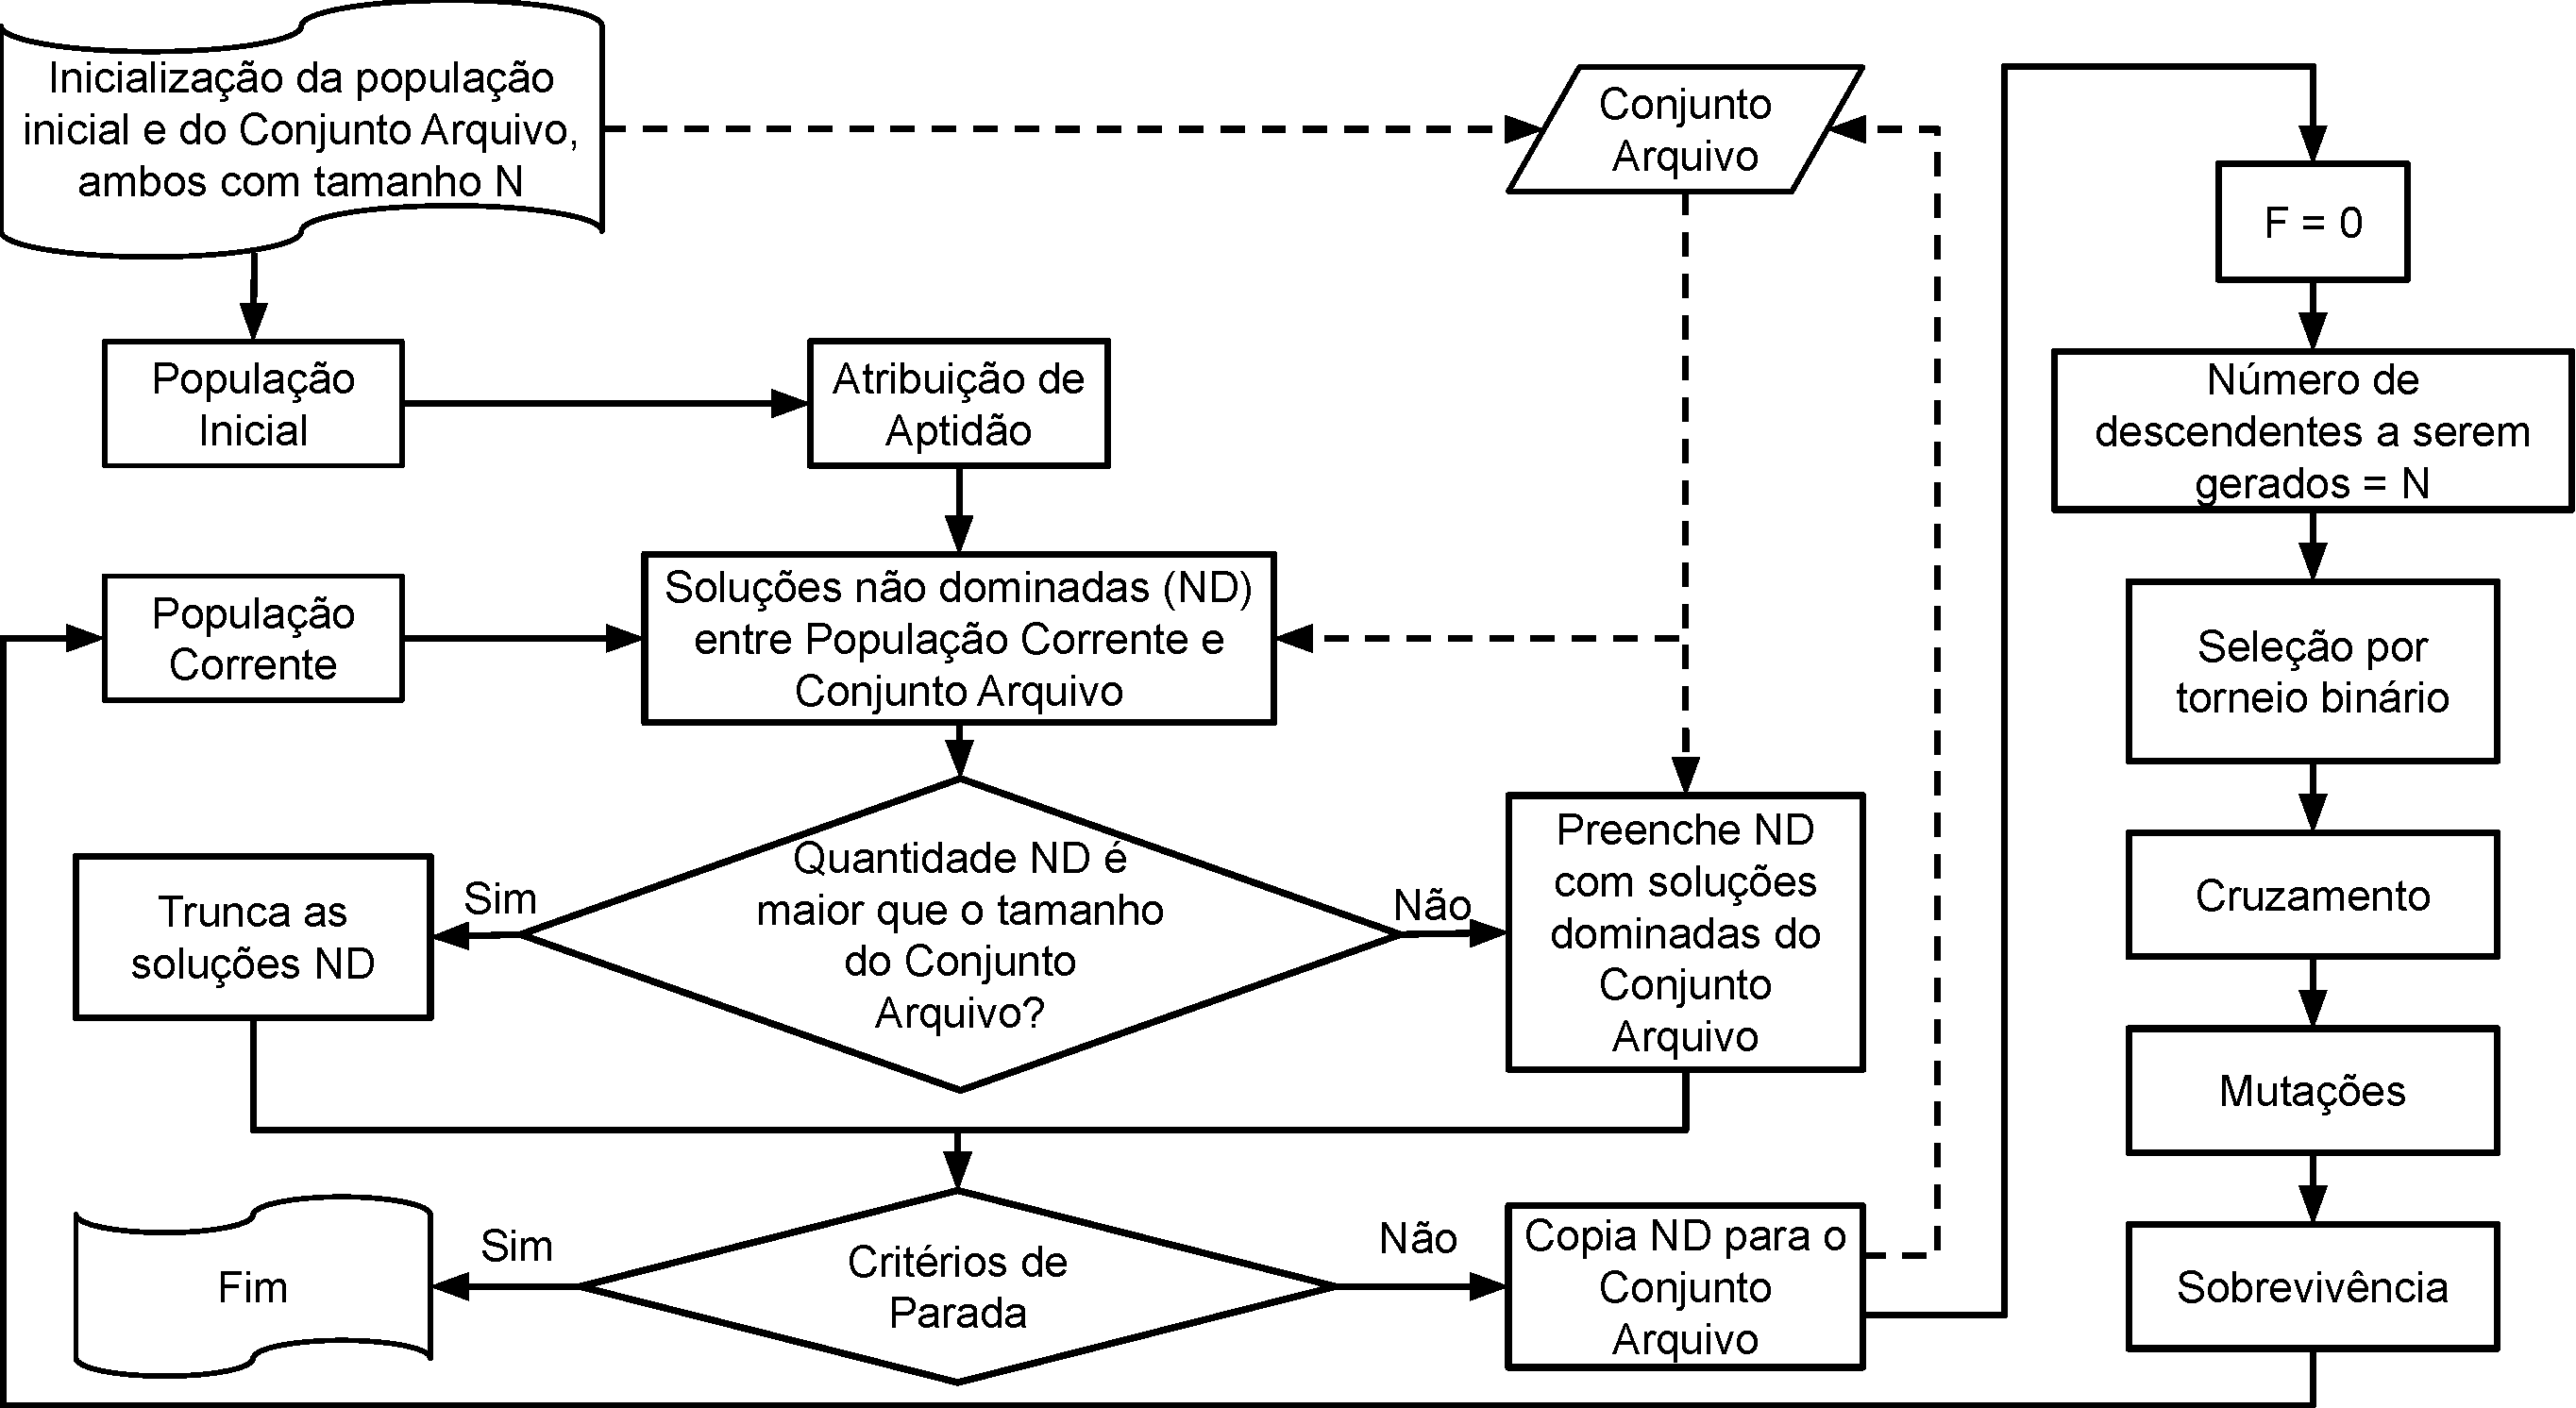
\includegraphics[width=0.8\textwidth]{fig/fluxo_spea2_pt.pdf}
\caption{Fluxograma do algoritmo SPEA2 mostrando as principais etapas de execução}
\label{fig:spea2_flow}
\end{figure}

Conforme apresentado na Figura~\ref{fig:spea2_flow}, o processo de evolução do SPEA2 pode ser resumido nos seguintes passos principais:

\begin{enumerate}
    \item \textbf{Inicialização:} A população inicial e o Conjunto Arquivo são inicializados, ambos com tamanho $N$. Esta etapa estabelece o ponto de partida para o processo evolutivo;
    
    \item \textbf{Atualização do Conjunto Arquivo:} Todos os indivíduos não dominados da população corrente $P_t$ e do Conjunto Arquivo $\bar{P}_t$ são identificados e copiados para formar um novo Conjunto Arquivo $\bar{P}_{t+1}$ para a próxima geração. Indivíduos dominados ou duplicatas (em termos de valores objetivo) são removidos durante esta operação;
    
    \item \textbf{Controle do tamanho do Conjunto Arquivo:} Se o número de soluções não dominadas for menor que o tamanho predefinido do Conjunto Arquivo, as posições restantes são preenchidas com as melhores soluções dominadas do Conjunto Arquivo anterior. Caso contrário, se o tamanho exceder o limite predefinido $\bar{N}$, os membros excedentes são removidos usando um método de truncamento que considera informações de densidade para preservar as características da fronteira não dominada;
    
    \item \textbf{Atribuição de aptidão:} Os valores de aptidão (baseados nas Equações~\ref{eq:strength_value}, \ref{eq:raw_fitness}, \ref{eq:density_estimation} e \ref{eq:final_fitness}) são calculados e atribuídos a todos os indivíduos tanto no Conjunto Arquivo quanto na população corrente;
    
    \item \textbf{Verificação dos critérios de finalização:} O algoritmo verifica se os critérios de parada foram atendidos (número máximo de gerações, convergência, etc.). Se atendidos, o processo é finalizado;
    
    \item \textbf{Seleção e reprodução:} Caso os critérios de finalização não sejam atendidos, operadores genéticos são aplicados para gerar a nova população $P_{t+1}$. A seleção por torneio binário é utilizada para escolher pais para reprodução, seguida pelos operadores de cruzamento e mutação para produzir $N$ descendentes que formarão a próxima geração.
\end{enumerate}

O fluxograma evidencia a natureza cíclica do algoritmo, onde o Conjunto Arquivo atua como um repositório elitista que preserva as melhores soluções encontradas ao longo do processo evolutivo, enquanto a população corrente é renovada a cada geração através dos operadores genéticos.

\subsection{Comparação com Outros MOEAs}

Ao comparar o SPEA2 com outros algoritmos evolutivos multi-objetivo notáveis, como o \textit{Non-dominated Sorting Genetic Algorithm II} (NSGA-II)~\cite{deb2002fast}, \textit{Multi-objective Particle Swarm Optimization} (MOPSO)~\cite{MOPSO} e \textit{Pareto Envelope-based Selection Algorithm II} (PESA-II)~\cite{PESA}, certas características distintivas se tornam evidentes.

Diferentemente do NSGA-II, o SPEA2 calcula explicitamente a força de cada indivíduo e utiliza um Conjunto Arquivo que está diretamente envolvido na avaliação da aptidão para todos os indivíduos. Enquanto o NSGA-II classifica suas soluções com base na ordenação por não dominância seguida pela distância de aglomeração (\textit{crowding distance}), a atribuição de aptidão do SPEA2 combina as relações de dominância de um indivíduo (via aptidão bruta $R(i)$) com uma medida de densidade baseada no $k$-ésimo vizinho mais próximo $D(i)$.

Comparado ao MOPSO, o SPEA2 adota uma abordagem mais tradicional da computação evolutiva, englobando operadores genéticos de cruzamento, mutação e seleção, em oposição à metodologia inspirada em enxames do MOPSO. Em contraste com a abordagem baseada em grade (\textit{grid-based}) do PESA-II para manter a diversidade, o SPEA2 preserva a diversidade populacional usando sua estimativa de densidade baseada no $k$-ésimo vizinho mais próximo.

Embora esses MOEAs possuam características únicas e vantagens específicas, a escolha entre eles frequentemente depende das particularidades do problema sendo abordado, incluindo o número de objetivos, dimensionalidade do espaço de busca e características da fronteira de Pareto.

O SPEA2 é reconhecido como um algoritmo robusto devido à sua capacidade de fornecer soluções de alta qualidade~\cite{zitzler2001spea2,citacaon1}. À medida que a otimização multi-objetivo se expande para diversos campos de aplicação, há uma demanda crescente por algoritmos de otimização mais eficazes~\cite{citacaon6}. No entanto, com o aumento da complexidade e escala dos problemas, torna-se necessário desenvolver abordagens eficientes que possam aproximar e distribuir soluções de forma mais rápida e eficaz próximo à fronteira de Pareto.

Diferentes técnicas podem ser incorporadas ou hibridizadas para contribuir com buscas locais ou globais, melhorando os resultados na resolução de problemas multi-objetivo. Uma abordagem promissora inclui a manutenção de um conjunto separado de soluções promissoras, como utilizado no próprio algoritmo SPEA2~\cite{zitzler2001spea2}. Algoritmos auxiliares também têm sido empregados para hibridizar algoritmos hospedeiros, intercalando buscas locais dentro do fluxo padrão de um algoritmo principal. Como exemplo de um algoritmo auxiliar usado nesses casos de hibridização, pode-se mencionar o método de Fertilização \textit{In Vitro} (IVF)~\cite{camilo-junior2011}.

\section{Hibridização de Algoritmos Evolutivos}
\label{sec:hibridizacao}

A hibridização de algoritmos evolutivos surgiu como uma abordagem fundamental para aprimorar o desempenho de técnicas de otimização em diversos domínios de problemas. Esta estratégia busca combinar características complementares de diferentes métodos para superar limitações individuais e melhorar tanto a qualidade das soluções obtidas quanto a eficiência computacional~\cite{talbi2002taxonomy}.

A integração de métodos distintos pode ocorrer de várias formas. Segundo Blum et al.~\cite{blum2011hybrid}, a hibridização pode ser classificada em três categorias principais: (i) \textbf{sequencial}, onde os algoritmos são aplicados um após o outro; (ii) \textbf{paralela}, com execução simultânea de diferentes algoritmos cooperando entre si; e (iii) \textbf{integrativa}, incorporando componentes específicos de um algoritmo dentro da estrutura de outro.

Talbi~\cite{citacaon2} propõe uma taxonomia mais abrangente para classificar hibridizações, considerando aspectos como nível de acoplamento (fraco ou forte), ordem de execução (sequencial ou paralela) e distribuição hierárquica dos algoritmos combinados. Esta taxonomia fornece um framework sistemático para o desenvolvimento e análise de algoritmos híbridos.

A combinação de algoritmos evolutivos com técnicas de busca local tem demonstrado resultados particularmente relevantes na literatura. Ishibuchi e Murata~\cite{ishibuchi1998multi} foram pioneiros nessa abordagem, propondo a integração sistemática de busca local em algoritmos genéticos multi-objetivo. Essa estratégia, posteriormente formalizada sob o termo ``algoritmos meméticos'', permite refinar soluções candidatas e acelerar a convergência para a fronteira de Pareto~\cite{knowles2000memetic}.

Estudos recentes demonstraram que abordagens híbridas podem superar significativamente algoritmos evolutivos convencionais em termos de qualidade da solução e velocidade de convergência~\cite{zhou2011multiobjective}. No entanto, o sucesso da hibridização depende criticamente da configuração adequada dos parâmetros de controle de ambos os algoritmos componentes e da estratégia de integração adotada~\cite{deb2012analyzing}. Além disso, é essencial considerar o equilíbrio entre exploração (\textit{exploration}) e explotação (\textit{exploitation}) para evitar convergência prematura ou perda de diversidade populacional.

\section{Método de Fertilização \textit{In Vitro}}
\label{sec:ivf}

O método de Fertilização \textit{In Vitro} (IVF)~\cite{camilo-junior2011} é um algoritmo auxiliar paralelo que pode ser integrado à fase de manipulação genética de um algoritmo hospedeiro, visando melhorar o desempenho do algoritmo original através da geração de indivíduos promissores. O IVF é inspirado no processo de reprodução assistida utilizado em laboratórios para produção de espécimes com características geneticamente superiores, funcionando como uma biotécnica reprodutiva aplicada para acelerar a produção de descendentes com propriedades desejáveis.

\subsection{Procedimento do Método IVF}

O funcionamento do método IVF segue um fluxo estruturado que permite sua integração harmoniosa com algoritmos evolutivos hospedeiros. A Figura~\ref{fig:ivf_flow} apresenta uma visão geral do processo, destacando as principais etapas de execução e suas interações.

\begin{figure}[htbp]
\centering
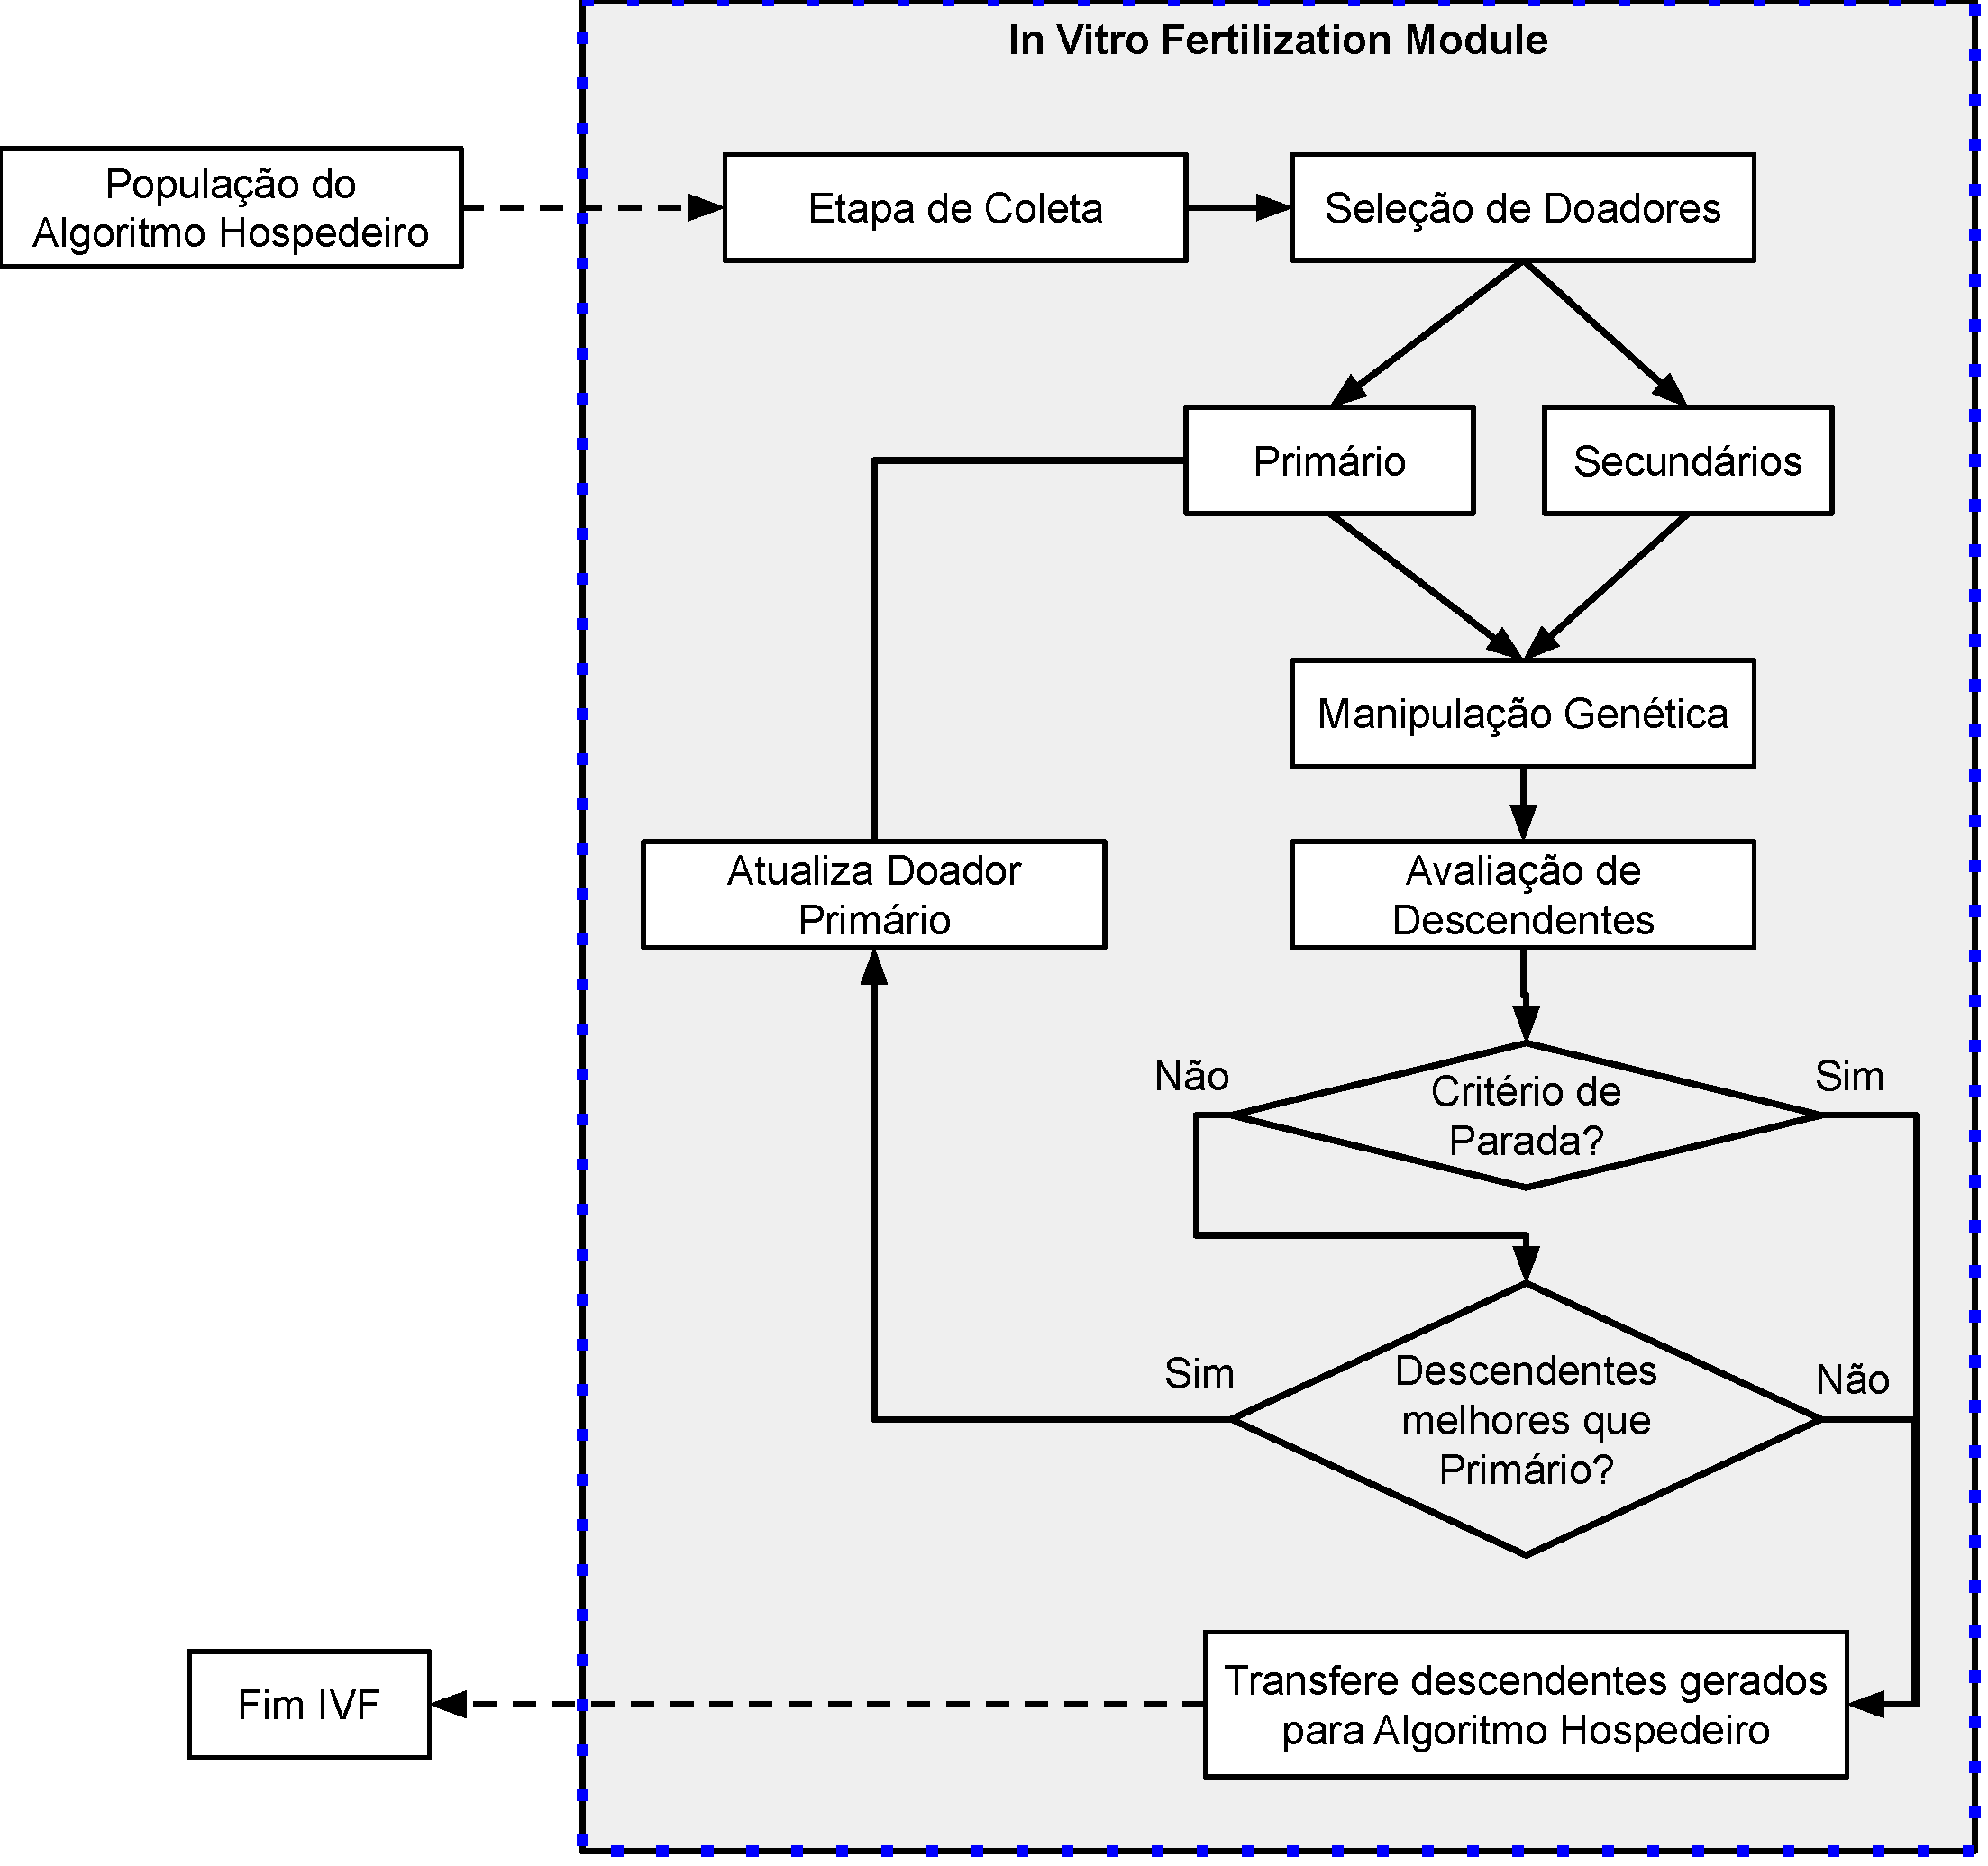
\includegraphics[width=0.7\textwidth]{fig/fluxo_ivf.pdf}
\caption{Fluxograma do método de Fertilização \textit{In Vitro} mostrando as etapas de coleta, manipulação genética e transferência}
\label{fig:ivf_flow}
\end{figure}

Conforme ilustrado na Figura~\ref{fig:ivf_flow}, o método IVF opera como um módulo independente que interage com o algoritmo hospedeiro através de três fases principais: coleta de material genético promissor, manipulação genética intensiva e transferência de descendentes superiores. O método IVF consiste nos seguintes passos principais:

\begin{enumerate}
    \item \textbf{Etapa de coleta:} Conforme mostrado na parte inicial do fluxograma, indivíduos promissores da população atual do algoritmo hospedeiro são coletados para manipulação genética. A seleção é baseada em critérios de qualidade definidos pelo problema, sendo que tipicamente $c$ indivíduos são coletados;
        
    \item \textbf{Separação de doadores:} O melhor indivíduo coletado é selecionado como o doador primário, enquanto os demais são designados como doadores secundários. Esta hierarquização permite direcionar as operações genéticas dentro do módulo de fertilização \textit{in vitro};
        
    \item \textbf{Manipulação genética:} Como destacado na figura, esta etapa central do processo aplica operações genéticas exploratórias, incluindo mutações direcionadas e cruzamentos elitistas, aos doadores coletados para criar descendentes com material genético promissor. O método IVF introduz variações controladas na composição genética, potencialmente gerando até $N$ indivíduos novos e superiores ($F \leq N$);
        
    \item \textbf{Avaliação da aptidão:} A aptidão dos descendentes é avaliada com base em seu desempenho nos objetivos do problema de otimização. Este passo fornece uma medida quantitativa da qualidade dos novos indivíduos gerados durante a manipulação genética;
        
    \item \textbf{Seleção de descendentes superiores:} Se um descendente superior emergir durante a fase de manipulação genética, superando a aptidão do doador primário atual, este indivíduo substitui o doador primário nas iterações subsequentes do método;
        
    \item \textbf{Critério de término:} Se nenhum descendente superar a aptidão do doador primário, ou outro critério de parada for atingido, o método IVF conclui suas iterações e prossegue para a fase de transferência;
        
    \item \textbf{Transferência:} Como ilustrado na etapa final da Figura~\ref{fig:ivf_flow}, um conjunto de $F$ descendentes superiores é transferido de volta para a população do algoritmo hospedeiro. Diferentes estratégias de transferência podem ser empregadas, incluindo a substituição de indivíduos menos aptos ou a expansão temporária da população.
\end{enumerate}

\subsection{Parâmetros de Controle}

O método IVF possui parâmetros específicos que controlam seu comportamento e integração com o algoritmo hospedeiro:

\begin{itemize}
    \item \textbf{Taxa de Execução ($r$):} Indica a probabilidade do método IVF ser acionado durante uma geração específica. Uma taxa mais alta resulta na execução do método IVF em um número maior de gerações, aumentando a intensidade da busca local;
    
    \item \textbf{Tamanho da Coleta ($c$):} Define o número de indivíduos coletados da população atual, incluindo o doador primário e os doadores secundários. Este parâmetro controla a diversidade genética disponível para manipulação.
\end{itemize}

\subsection{Operadores de Recombinação}

O método IVF emprega diferentes operadores de recombinação para explorar o espaço de busca de forma eficiente~\cite{camilo-junior2011}:

\begin{itemize}
    \item \textbf{Recombinação Assistida (AR):} Utiliza informações da população do algoritmo genético hospedeiro, aumentando a velocidade da operação sem realizar alterações genéticas significativas;
    
    \item \textbf{Recombinação Assistida Exploratória com Novos indivíduos (EAR-N):} Diversifica o espaço de busca substituindo metade dos doadores secundários por novos indivíduos gerados aleatoriamente;
    
    \item \textbf{Recombinação Assistida Exploratória Total (EAR-T):} Aplica mutação ao cromossomo completo de metade dos doadores secundários coletados, promovendo exploração ampla;
    
    \item \textbf{Recombinação Assistida Exploratória Parcial (EAR-P):} Realiza mutação em apenas parte do cromossomo dos doadores secundários, permitindo exploração localizada;
    
    \item \textbf{Recombinação Assistida Exploratória Parcial Adaptativa (EAR-PA):} Instiga mutação cromossômica parcial adaptativa em alguns indivíduos de metade dos doadores secundários, ajustando a intensidade da exploração conforme necessário.
\end{itemize}

Essas diferentes configurações de operadores permitem examinar sistematicamente a influência do método IVF no desempenho do algoritmo hospedeiro, possibilitando ajustes finos para diferentes tipos de problemas e características da fronteira de Pareto.